%label:"rem:heegaardStabilizations"
%author:JeffHicks
%name:"Morse interpretation of Heegaard stabilization"
%type:"remark"
%parent:"def:heegaardStabilization"

One way to see that stabilization of a Heegaard diagram produces the same manifold comes from Morse theory. Consider $\Sigma_g$ as the level set of a self-indexing Morse function $f$. Suppose that we wanted to modify our Morse function to $\tilde f$ by adding in a pair of critical points $p, q$ so that $\ind(p)=1$ and $\ind(q)=2$. We imagine that the critical points would appear on opposite sides of $\Sigma_g$, and be connected by a single flow line. Furthermore, $\tilde \Sigma_{g+1}=\tilde f(1.5)$, the new level set, would be of genus $g+1$. By applying surgery along either the attaching circles $W^\downarrow(p)\cap \tilde \Sigma_{g+1}$ or $W^\uparrow(q)\cap \tilde \Sigma_{g+1}$, we obtain $\Sigma_g$. See \cref{fig:heegaardStabilization}.
%label:"fig:heegaardStabilization"
%author:JeffHicks
%name:"rounding corner in Polterovich surgery"
%type:"figure"
%parent:"thm_roundingCorner"
%caption:"From the perspective of Morse theory, stabilization comes from the creation of a pair of cancelling critical points."



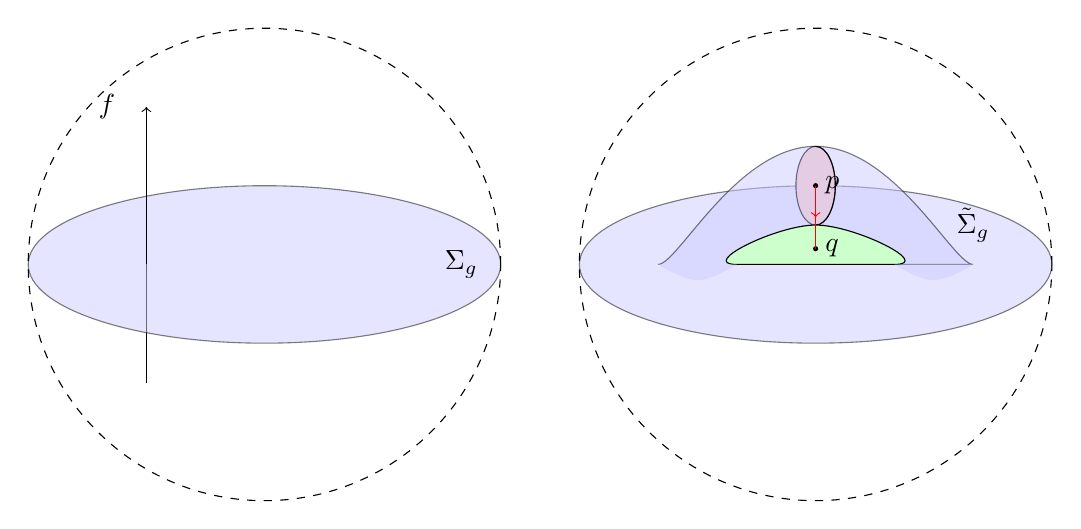
\begin{tikzpicture}
    \draw (-4,-1) -- (-4,0.5) ;
    \draw[opacity=.5,fill= blue!20]  (-2.5,0.5) ellipse (3 and 1);
    \draw[opacity=.5, fill=blue!20]   (4.5,0.5) node (v1) {} ellipse (3 and 1);
    \draw (6,-2);
    \draw[->](-4,0.5) -- (-4,2.5);
    \node at (-4.5,2.5) {$f$};
    \node at (0,0.5) {$\Sigma_g$};
    \draw[dashed]  (-2.5,0.5) ellipse (3 and 3);
    \draw[dashed]  (v1) ellipse (3 and 3);
    \draw[fill=red!20]  (4.5,1.5) ellipse (0.25 and 0.5);
    \draw[opacity=.5, fill=blue!20] (2.5,0.5) .. controls (2.75,0.5) and (3.5,2) .. (4.5,2) .. controls (5.5,2) and (6.25,0.5) .. (6.5,0.5) .. controls (6.25,0.5) and (6.25,0.5) .. (5.5,0.5) .. controls (5.75,0.5) and (5,1) .. (4.5,1) .. controls (4,1) and (3.25,0.5) .. (3.5,0.5);
    
    \node[right] at (4.5,1.5) {$p$};
    \node[fill=black, circle, scale=.2] at (4.5,1.5) {};
    \begin{scope}[]
    
    \clip  (5,1) rectangle (4.5,2);
    \draw  (4.5,1.5) ellipse (0.25 and 0.5);
    \end{scope}
    
    
    
    \draw[fill=green!20] (3.5,0.5) .. controls (3,0.5) and (4,1) .. (4.5,1) .. controls (5,1) and (6,0.5) .. (5.5,0.5)--cycle;
    \node[right] at (4.5,0.7) {$q$};
    \node[circle, fill=black, scale=.2] at (4.5,0.7) {};
    
    \begin{scope}[]
    
    \fill[opacity=.5, fill=blue!20]  plot[smooth, tension=.7] coordinates {(2.5,0.5) (3,0.3) (3.5,0.5)};
    
    \end{scope}\begin{scope}[shift={(3,0)}]
    
    \fill[opacity=0.5, fill=blue!20]  plot[smooth, tension=0.7] coordinates {(2.5,0.5) (3,0.3) (3.5,0.5)};
    
    \end{scope}\node at (6.5,1) {$\tilde \Sigma_g$};
    
    \draw[red,->] (4.5,1.5) -- (4.5,1.1);
    \draw[red] (4.5,1.1) -- (4.5,0.7);
    \end{tikzpicture}
